%!TEX root = ../report.tex
\chapter{Methodology}

In line with the goal of the project to use resource efficient deep learning in terms of inference time and storage memory, the deepLab v3+ model with mobileNetv2 and Xception variant was chosen. In order to better understand deepLabv3+, we consider breaking down the architectures of the previous versions of deepLab leading upto the current version. The different versions of deepLab are deepLab, deepLabv2, deepLabv3 and deepLabv3+ (the current version also called as deepLabv4). Also, we review the pruning and quantization methods considered for this work.

\section{DeepLab}

Fully Convolutional networks were introduced by [] for the task of semantic segmentation. The predictions obtained with the help of this network were coarse and the object boundaries were not sufficiently delineated. In order to overcome these difficulties, the authors of deepLab proposed the use of atrous convolutions and fully-connected Conditional Random Fields (CRF).

Atrous convolutions, also called as dilated convolutions, is used to gather a better global context with enlarged field-of-view on the feature maps. An atrous rate "r", determines the field-of-view of an atrous convolution. With increase in atrous rate, a greater region of a feature map is convolved over. This leads to gathering of more global context. However, it is worth noting that there is no increase in the number of parameters in the convolution filter. Only the convolved region in the input feature map changes. When the atrous rate is 1, standard convolution is performed. The Figure \ref{Fig:atconv} illustrates atrous convolution. 

	\begin{figure}
		\begin{subfigure}{.3\textwidth}
			\centering
			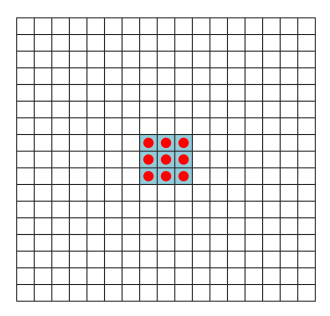
\includegraphics[width=1.03\linewidth]{images/r_1}
			\caption{Atrous rate = 1}
		\end{subfigure}
		\begin{subfigure}{.3\textwidth}
			\centering
			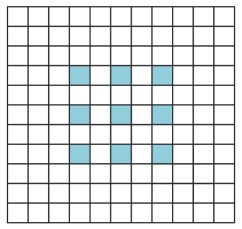
\includegraphics[width=1\linewidth]{images/r_2}
			\caption{Atrous rate = 2}
		\end{subfigure}
		\begin{subfigure}{.3\textwidth}
			\centering
			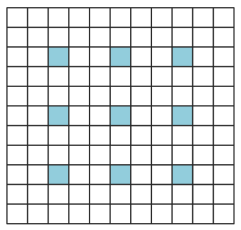
\includegraphics[width=1\linewidth]{images/r_3}
			\caption{Atrous rate = 3}
		\end{subfigure}
		\caption{Illustration of atrous convolution with three different atrous rates.}
		\label{Fig:atconv}
	\end{figure}
	
Fully-connected Conditional Random Fields (CRF), is used to post process the prediction of the segmentation network used in deepLab, to improve object delineation. Every pixel in the output feature map is connected to every other pixel resulting in pairwise terms. In each pairwise term, based on color and position, the similarity between pixels is determined and a class is assigned for the pixels.


\section{DeepLabv2}

% Source: http://www.davidtvs.com/exploring-semantic-segmentation-dnn/
In DeepLabv2, Atrous Spatial Pyramid Pooling (ASPP) was used in addition to the existing architecture. The authors also use deeper ResNet network to improve accuracy.

Atrous Spatial Pyramid Pooling, is used to create multiscale feature representations. Atrous convolutions with different atrous rates are applied to the same feature map. The resulting feature maps from each atrous convolution is processed in separate branches in a similar fashion as in deepLabv1 by using two 1$\times$1 convolutions. Each of the branches are then fused together to obtain multiscale information. The difference between in architecture between deepLabv1 and deepLabv2 is illustrated in \ref{Fig:v1vsv2}.

	\begin{figure}
		\centering
		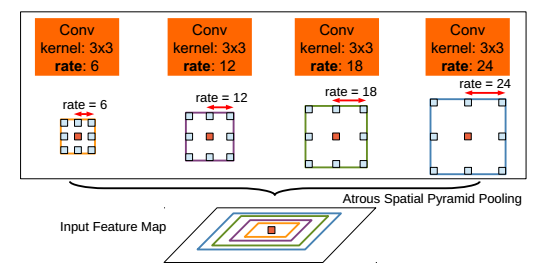
\includegraphics[width=0.6\linewidth]{images/aspp}
		\caption{Illustration of Atrous Spatial Pyramid Pooling (ASPP). Atrous convolutions with 4 different rates convolve on the same input feature map. The field-of-view of each atrous rate is shown using different colors.}
		\label{Fig:aspp}
	\end{figure}
	
	\begin{figure}
		\begin{subfigure}{.5\textwidth}
			\centering
			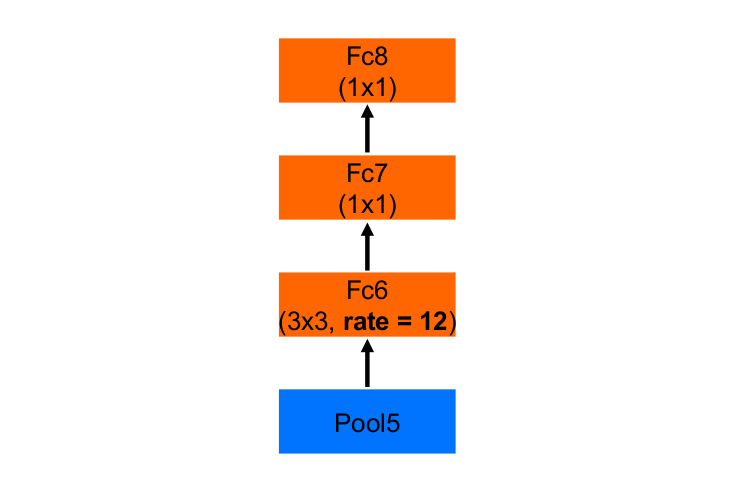
\includegraphics[width=1.03\linewidth]{images/v1_largeFOV}
			\caption{Large field-of-view in DeepLabv1}
		\end{subfigure}
		\begin{subfigure}{.5\textwidth}
			\centering
			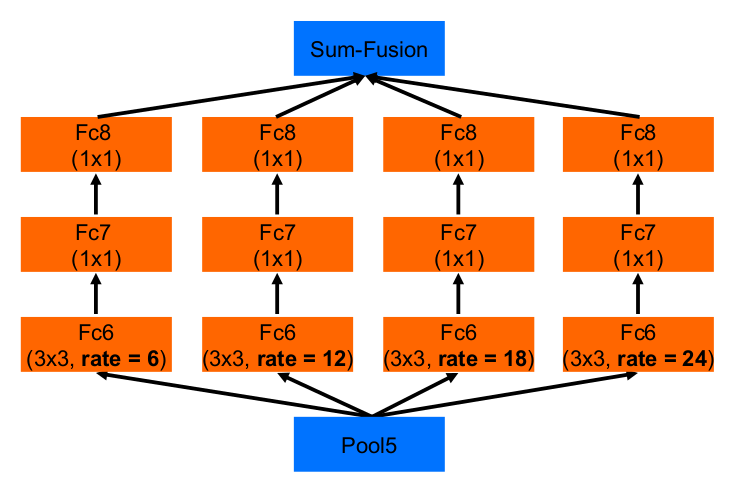
\includegraphics[width=1\linewidth]{images/v2_aspp}
			\caption{ASPP in DeepLabv2}
		\end{subfigure}
		\caption{Illustration of the difference in architecture between DeepLabv1 and DeepLabv2.}
		\label{Fig:v1vsv2}
	\end{figure}
	
\section{DeepLabv3}
In this version of deepLab, the contributions include improvements to the context module, and the use of batch normalization. Batch Normalization is applied to every layer in the context module and the parameters of the batch normalization layers are trained.

The authors experiment with two different modules to handle context one being a cascade module and the other being an improved version of ASPP module. The cascade module is formed by repeating the last block from ResNet and replacing convolutions with atrous convolutions. The authors report that performing this repetition upto three times improves performance. 	The cascade module is illustrated in \ref{Fig:contextmodulea}. The ASPP module used in deepLabv3 is similar to the one used in deepLabv2. However, the difference now is that the ASPP module uses five branches. The first four branches perform 1$\times$1 convolution, and three 3$\times$3 convolutions with atrous rates 6, 12 and 18. The 5th branch provides image level features by performing global average pooling on the last feature maps of the model. The resulting channels are concatenated and projected to a different channel space using 1$\times$1 convolution.

	\begin{figure}
		\begin{subfigure}{1\textwidth}
			\centering
			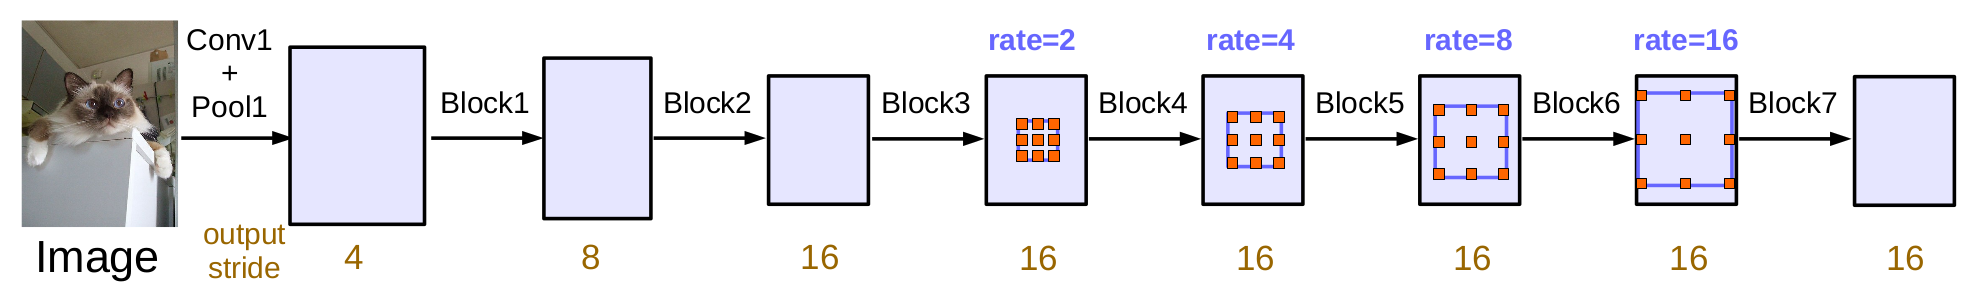
\includegraphics[width=1\linewidth]{images/cascade_module}
			\caption{cascade module in DeepLabv3}
			\label{Fig:contextmodulea}
		\end{subfigure}
		\begin{subfigure}{1\textwidth}
			\centering
			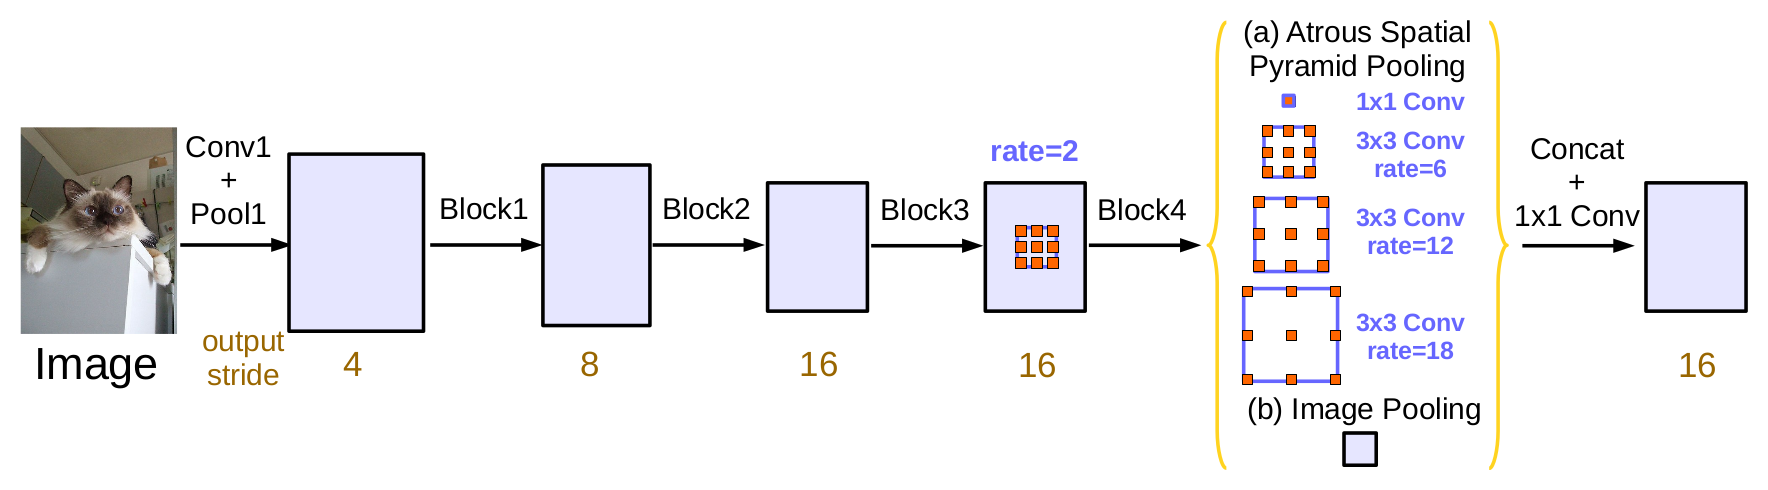
\includegraphics[width=1\linewidth]{images/aspp_module}
			\caption{ASPP module in DeepLabv3}
			\label{Fig:contextmoduleb}
		\end{subfigure}
		\caption{Illustration of two different context modules used in deepLabv3.}
		\label{Fig:contextmodule}
	\end{figure}

\section{DeepLabv3+}

DeepLabv3+ is designed to combine the ability of ASPP module which can capture rich context information and the ability of encoder-decoder networks which can produce sharp object boundary delineation. Xception, mobileNetv2 and ResNet-101 are used as encoders out of which this work only considers xception and mobileNetv2 for their resource efficiency. The major differences in deepLabv3+ is the use of a decoder, the use of atrous separable convolutions in both the encoder and decoder and the adaption of mobileNet and xception as network backbones (encoders).

The authors call the ratio of input resolution to the output resolution before global average pooling as the output stride. DeepLabv3 is designed to have an output stride of 16. To bring the prediction to the original image resolution, the final features are upsampled by using bilinear interpolation by a factor of 16. This is considered by the authors as a naive decoder module. Instead of this naive approach, the authors propose the use of a better decoder module. The final encoder features are first upsampled by a factor of 4, and are concatenated with the low level features from the encoder with same dimensions. The number of channels in the low level features are first reduced using a 1$\times$1 convolution. A 3$\times$3 convolution convolves over this concatenated features to refine the features and is later followed by an upsampling of 4 to lead to the final prediction. The architecture of deepLabv3+ is depicted in \ref{Fig:deepLabv4}.

	\begin{figure}
		\centering
		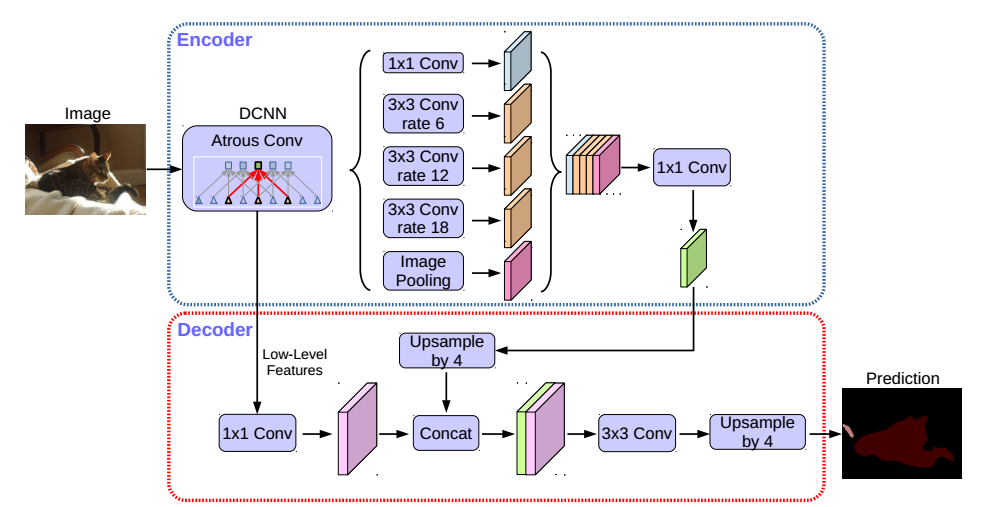
\includegraphics[width=1\linewidth]{images/deepLabv4}
		\caption{An illustration of deepLabv3+ architecture. The encoder extracts features at different scales and the decoder refines object boundary delineation.}
		\label{Fig:deepLabv4}
	\end{figure}

The mobileNetv2 and xception encoders make use of depthwise separable convolutions to improve resource efficiency. Sections \ref{section:mn} and \ref{section:xcep} provide details regarding mobileNetv2 and xception architectures respectively. In deepLabv3+, the authors use atrous convolution instead of depthwise convolution in depthwise seperable convolution. The authors call this type of convolutions as atrous separable convolution and state that these convolutions can be used to extract feature maps at arbitrary resolution. The authors use a modified version of the xception architecture as depicted in \ref{Fig:deepLabv4_xcep} as one of the network backbones.

	\begin{figure}
		\centering
		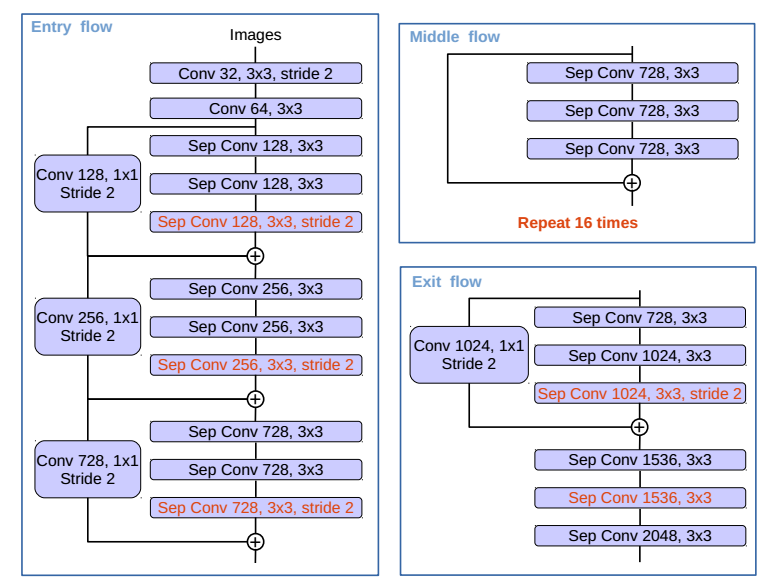
\includegraphics[width=.8\linewidth]{images/deepLabv4_xcep}
		\caption{Modified xception architecture used as encoder in deepLabv3+. The max pooling operations in the original xception architecture are replaced with depthwise separable convolutions. Batch normalization and ReLU activation is applied after each 3$\times$3 depthwise convolution.}
		\label{Fig:deepLabv4_xcep}
	\end{figure}

\section{MobileNetv2}
\label{section:mn}

% to cite: https://towardsdatascience.com/mobilenetv2-inverted-residuals-and-linear-bottlenecks-8a4362f4ffd5

% mobileNetv2 building block: https://ai.googleblog.com/2018/04/mobilenetv2-next-generation-of-on.html 

% depthwise : https://eli.thegreenplace.net/2018/depthwise-separable-convolutions-for-machine-learning/

The mobileNetv2 architecture is designed to work on mobile and embedded devices where computational resources are limited. The authors state that their main contribution is the use of a novel layer module called the inverted residual with linear bottleneck. 

Depthwise separable convolutions, known for its efficiency, is used in this work. Standard convolution layers are replaced with two layers where the first layer performs depthwise convolution and the second layer performs pointwise convolution. A depthwise convolution layer uses a single fiter per input channel to perform convolution. The pointwise convolution layer consists of 1$\times$1 convolutions which perform weighted linear combination on the input channels and project them to a new channel space. This factorization of standard convolution layer into two separate depthwise and pointwise layers leads to roughly $k^2$ times reduction in computation cost where k is the kernel size of the convolutional filter. Figure \ref{Fig:depthwise} illustrates depthwise convolution. In this case, pointwise convolution performs dimensionality reduction as the number of output channels is less than number of input channels. However, in this case, if more than 3 pointwise convolutions are used, dimensionality output channels can be increased.

	\begin{figure}
		\centering
		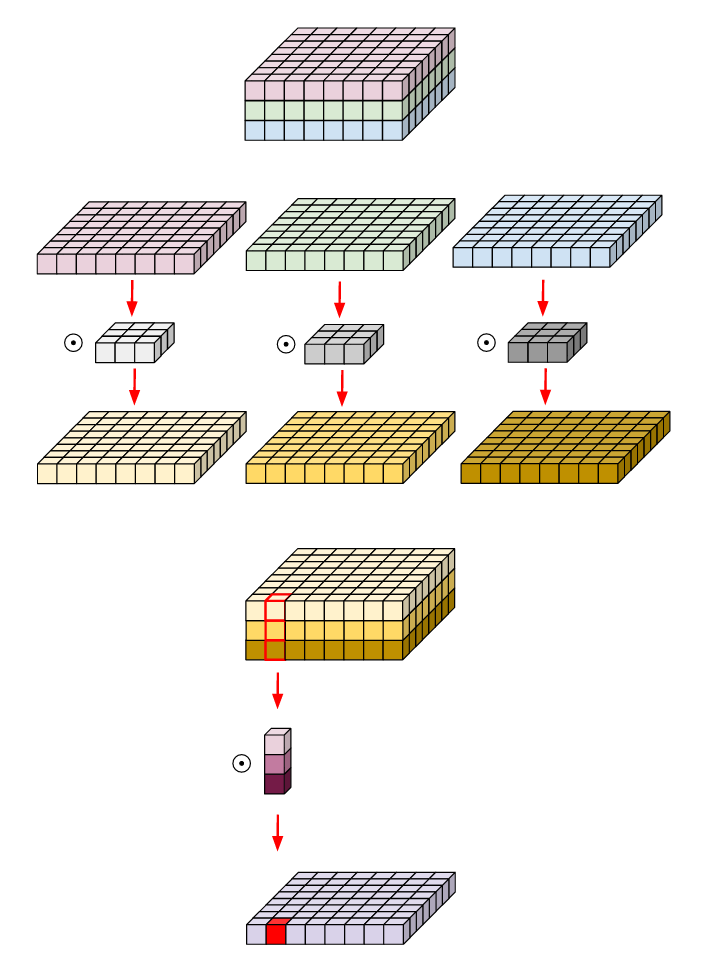
\includegraphics[width=.5\linewidth]{images/depthwise}
		\caption{An illustration of depthwise separable convolution with 3 input channels and 1 output channel. The first row shows the three input channels. The next three rows illustrate three separate 3$\times$3 convolution convolving over one of the input channels. The fifth row shows the resulting feature maps of the three convolutions being stacked upon each other. Rows 2 to 5 together is the depthwise convolution. The sixth row shows a pointwise convolution convolving over the output of depthwise convolution to get the final output channel}
		\label{Fig:depthwise}
	\end{figure}

In the original residual block [cite], first a 1$\times$1 convolution is used to reduce the number of channels. On this reduced number of channels 3$\times$3 standard convolution is done which is followed by a 1$\times$1 convolution which now expands the feature maps to have the same number of channels as the input to the block. A skip connection is then introduced through which the input channels is added to the output channels of the residual block. The skip connection provides a layer with access to earlier activations and also helps prevents the vanishing gradients problem. 

The authors of mobileNetv2 propose the use of inverted residual block which takes advantage of the depthwise seperable convolutions. This block consists of a narrow bottleneck layer followed by a 1$\times$1 convolution which performs expansion of number of channels. Depthwise convolution is performed on the expanded input channels followed by a pointwise convolution which brings down the number of channels to create the next bottleneck layer. A skip connection is then added between the input bottleneck and the output bottleneck. The original and inverted residual blocks are depicted in \ref{Fig:residual}. The authors use linear activation in the bottleneck layers and hypothesize that it is better than non-linear activation.

	\begin{figure}
		\begin{subfigure}{.5\textwidth}
			\centering
			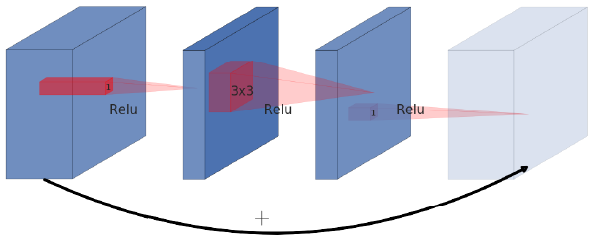
\includegraphics[width=.8\linewidth]{images/residual}
			\caption{Residual block}
		\end{subfigure}
		\begin{subfigure}{.5\textwidth}
			\centering
			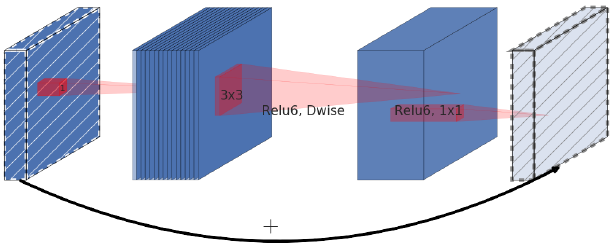
\includegraphics[width=.8\linewidth]{images/inverted_residual}
			\caption{Inverted residual block}
		\end{subfigure}
		\caption{Illustration of the original residual block and the inverted residual block used by mobileNetv2.}
		\label{Fig:residual}
	\end{figure}

This hypothesis is based on the notion that the ReLU activation layer used, leads to information loss due to loss of values less than 0. However, loss of too much information due to the induced nonlinearity by the activation can be prevented by the use of linear activation in the bottleneck layer. The authors show that a linear activation is empirically better than a non linear activation in the bottleneck layer.

The inverted residual block has less number of parameters than the residual block and with linear bottleneck is shown to achieve state-of-the-art performance. The inverted residual block is visualized in the architecture of mobileNetv2 in \ref{Fig:mobileNetv2bb}.

	\begin{figure}
		\centering
		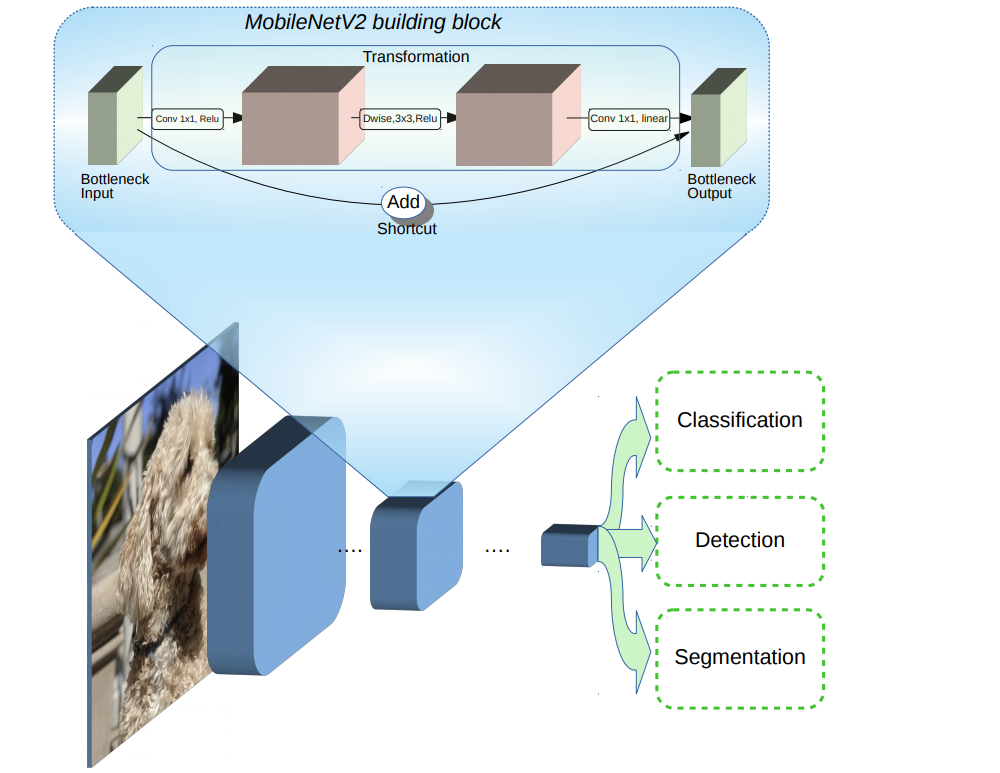
\includegraphics[width=.7\linewidth]{images/mobileNetv2_bb}
		\caption{The building block of mobileNetv2. The compressed representation obtained could be used for tasks such as image classification, object detection and semantic segmentation.}
		\label{Fig:mobileNetv2bb}
	\end{figure}

\section{Xception}
\label{section:xcep}

The xception architecture is derived based on two hypothesis made by the authors. One hypothesis is based on the inception architecture and the other is a stronger version of the inception hypothesis. Standard convolution layers has 3D convolution kernals which maps both spatial correlations and cross-channel correlations at the same time. Here spatial correlations is obtained by mapping correlations across the height and the width of every channel separately. Cross-channel correlations is obtained at every spatial location across the height and width of the channels, from each of the channels in the input. 

In the inception architecture, an inception module consists of 4 branches operating on the same input feature maps. The different branches of the inceptionv3 module is shown in \ref{Fig:xceptiona}. In the second branch with 1$\times$1 convolution followed by a 3$\times$3 convolution, the 1$\times$1 convolution calculates the cross-channel correlation between the input channels and performs dimensionality reduction by reducing the number of input channels. Next, the 3$\times$3 convolution is a standard convolution which looks for both spatial and cross-channel correlations in this reduced input channel space. Since this inception module has lead to state-of-the-art classification results, the authors hypothesize that the cross-channel correlations and spacial correlations are decoupled and can be mapped separately. This is evidently based on the fact that the inception module partially handles spatial and cross-channel correlations in a decoupled fashion by using a 1$\times$1 convolution followed by a 3$\times$3 convolution. 

	\begin{figure}
		\begin{subfigure}{.5\textwidth}
			\centering
			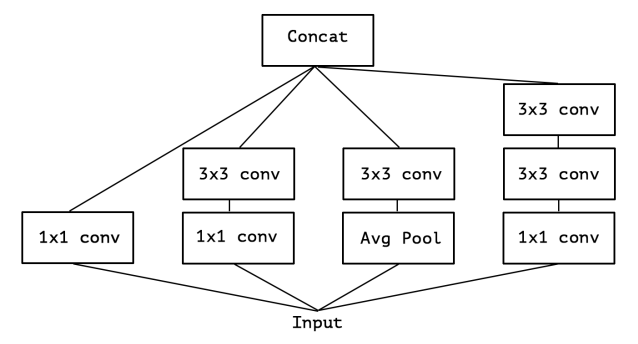
\includegraphics[width=.8\linewidth]{images/inception_v3}
			\caption{Inceptionv3 module}
			\label{Fig:xceptiona}
		\end{subfigure}
		\begin{subfigure}{.5\textwidth}
			\centering
			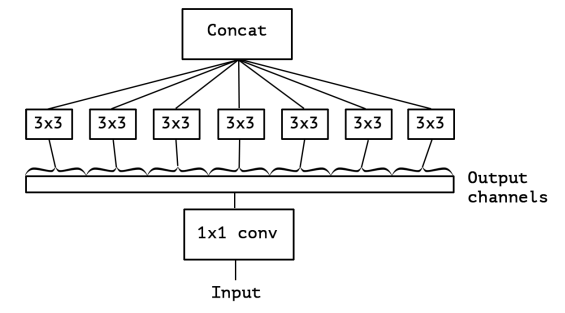
\includegraphics[width=.8\linewidth]{images/extreme_inception}
			\caption{Extreme version of inception module}
			\label{Fig:xceptionb}
		\end{subfigure}
		\caption{Illustration of the inception v3 module and an extreme version of the inception module. In the extreme version, each of the 3$\times$3 convolution operates on a single output channel of 1$\times$1 convolution.}
		\label{Fig:xception}
	\end{figure}

Based on this hypothesis, the authors propose that the two correlations can be mapped completely independent of each other leading to a stronger hypothesis. An illustration of this stronger hypothesis can be seen in \ref{Fig:xceptionb}. The xception network is based on this stronger hypothesis and is named "xception" as the architecture is a extreme version of inception. The complete decoupling of the two correlations, could be obtained using depthwise separable convolution, as evidently, this type of convolution first performs depthwise convoltion which handles the spatial correlation and then performs pointwise convolution which handles cross-channel correlation.

\section{Pruning}

A trained Deep Convolutional Neural Network (DCNN) might have weights which are redundant in terms of its effect on the performance during inference.

\section{Quantization}
